\documentclass{article}

\usepackage{graphicx} % Para inserir imagens
\usepackage{lipsum}   % Para gerar texto de exemplo (remova ou substitua pelo seu conteúdo)
\usepackage{fancyhdr}
\usepackage{lastpage}
\usepackage{titlesec} % Pacote para personalizar títulos de seções
\usepackage{csvsimple}

% Configuração do estilo da página
\fancypagestyle{plain}{% Estilo da primeira página
  \fancyhf{} % Limpa os cabeçalhos e rodapés
  \fancyhead[L]{\vspace*{-2cm}
\includegraphics[width=4cm]{Picture1.png}} % Imagem no cabeçalho
  \fancyhead[R]{\thepage/\pageref{LastPage}} % Número da página no cabeçalho
  \fancyfoot[R]{\vspace*{+1cm}
\includegraphics[width=8cm]{Picture2.png}} % Imagem no rodapé
  \renewcommand{\headrulewidth}{0pt} % Remove a linha horizontal do cabeçalho
  \renewcommand{\footrulewidth}{0pt} % Remove a linha horizontal do rodapé
}
\pagestyle{fancy}
\fancyhf{} % Limpa os cabeçalhos e rodapés
\fancyhead[L]{\vspace*{-2cm}
\includegraphics[width=4cm]{Picture1.png}} % Imagem no cabeçalho
\fancyhead[R]{\thepage/\pageref{LastPage}} % Número da página no cabeçalho
\fancyfoot[R]{\vspace*{+1cm}
\includegraphics[width=8cm]{Picture2.png}} % Imagem no rodapé
\renewcommand{\headrulewidth}{0pt} % Remove a linha horizontal do cabeçalho
\renewcommand{\footrulewidth}{0pt} % Remove a linha horizontal do rodapé

% Estilo para alinhar à esquerda
\titleformat{\section}[hang]{\bfseries\Large}{\thesection}{1em}{}

\begin{document}
\thispagestyle{plain} % Aplica o estilo de página customizado à primeira página
\title{\textbf{MONITORAMENTO SISMOLÓGICO} \\
\textbf{RSIS - Rede Sismológica Itá/Machadinho, SC/RS} \\
\textbf{Reservatório de Machadinho, SC/RS} \\
\textbf{BOLETIM SÍSMICO Nº XXXXXX}}
\maketitle

\section{PERÍODO DE ANÁLISE:}

\section{ÚLTIMOS RELATÓRIOS TÉCNICOS:}

\section{ATIVIDADES REALIZADAS:}

\section{RESULTADOS:}

\section{CONSIDERAÇÕES:}

\newpage
% Seção alinhada à esquerda
\titleformat{\section}[hang]{\bfseries\Large}{\thesection}{1em}{} % Ajusta o alinhamento à esquerda
\section{COMPLETEZA DOS DADOS}
\begin{figure}[h]
    \centering
    \caption{Gráfico de completeza dos dados para o mês de XXX para estação XXX}
    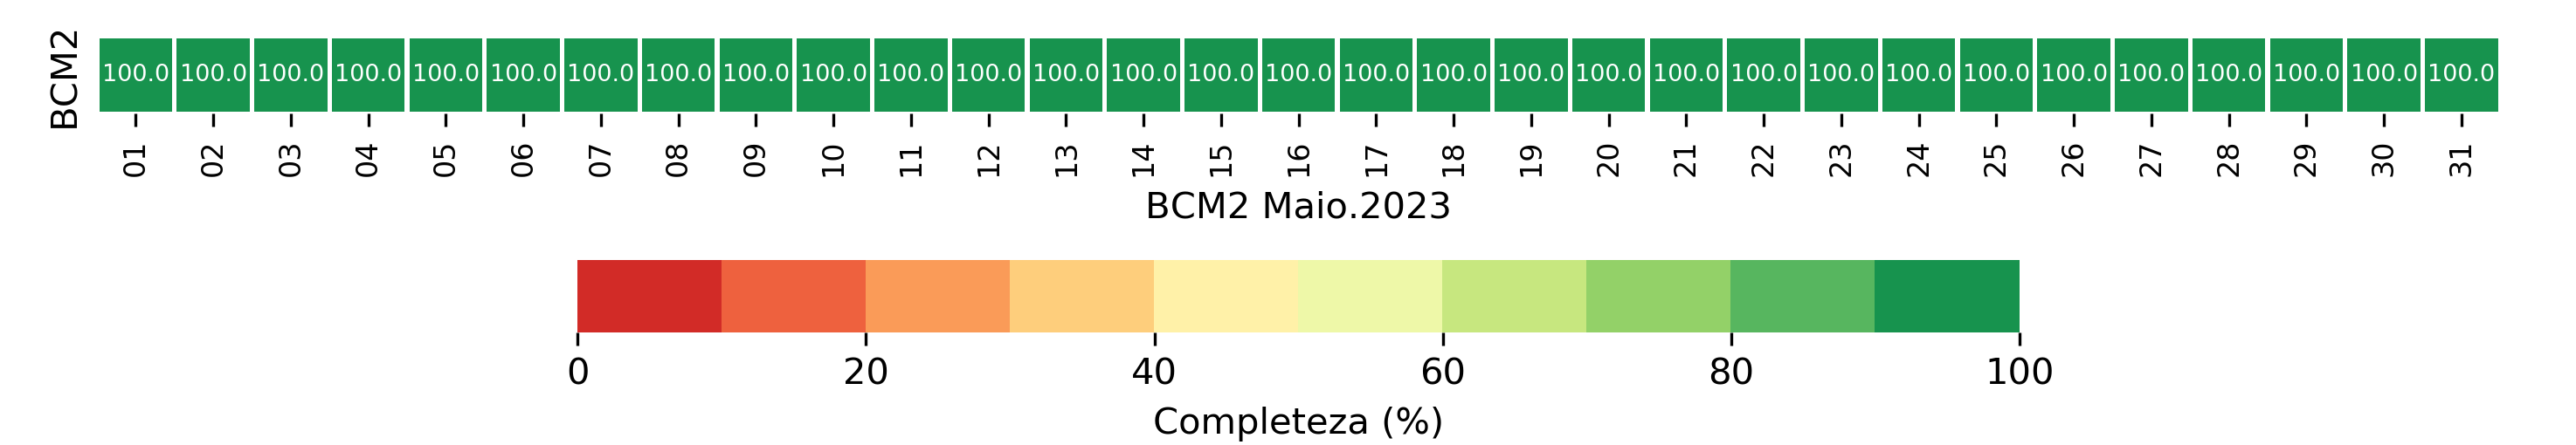
\includegraphics[width=1.2\textwidth]{completeza_dos_dados.png} % Substitua pelo nome da imagem e ajuste o tamanho
\end{figure}
Fonte: IPT

\section{TABELA DE EVENTOS}
\csvautotabular{events-2023-06-01-IT_virgulas.csv}

% Restante do conteúdo

\newpage
\begin{thebibliography}{9}
  \bibitem{ref1} Autor1. \emph{Título da Referência 1}. Editora, Ano.
  \bibitem{ref2} Autor2. \emph{Título da Referência 2}. Editora, Ano.
  % Adicione suas referências bibliográficas aqui
\end{thebibliography}

\end{document}

